\hypertarget{stack_8c}{
\section{stack.c File Reference}
\label{stack_8c}\index{stack.c@{stack.c}}
}
{\tt \#include \char`\"{}stack.h\char`\"{}}\par


Include dependency graph for stack.c:\begin{figure}[H]
\begin{center}
\leavevmode
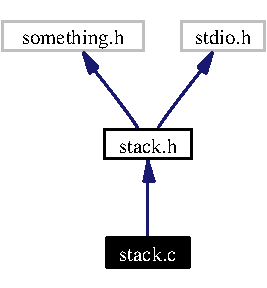
\includegraphics[width=81pt]{stack_8c__incl}
\end{center}
\end{figure}
\subsection*{Functions}
\begin{CompactItemize}
\item 
int \hyperlink{group__stack_a0}{push} (\hyperlink{structstack}{stack} s, int val)
\begin{CompactList}\small\item\em This function is used to push stuff.\item\end{CompactList}\item 
int \hyperlink{stack_8c_a1}{pop} (\hyperlink{structstack}{stack} s, int val)
\end{CompactItemize}


\subsection{Detailed Description}




Definition in file \hyperlink{stack_8c-source}{stack.c}.

\subsection{Function Documentation}
\hypertarget{stack_8c_a1}{
\index{stack.c@{stack.c}!pop@{pop}}
\index{pop@{pop}!stack.c@{stack.c}}
\subsubsection[pop]{\setlength{\rightskip}{0pt plus 5cm}int pop (\hyperlink{structstack}{stack} {\em s}, int {\em val})}}
\label{stack_8c_a1}


\begin{Desc}
\item[\hyperlink{todo__todo000001}{Todo: }]\par
 Impliment this function \end{Desc}
 \begin{Desc}
\item[Examples: ]\par
\hyperlink{stack__example_8c-example}{stack\_\-example.c}.\end{Desc}


Definition at line 24 of file stack.c.